\documentclass[11pt]{article}
\usepackage{graphicx}
\usepackage[margin=1in]{geometry} %reducir márgenes
\usepackage{cite} %opciones entre {}
\pagestyle{empty} %quitar números de página
\usepackage{enumerate}

\setlength{\parskip}{8mm}

\parindent 0ex 
\renewcommand{\baselinestretch}{1.2} 

\begin{document}

\section*{\textbf{Reports Zenhub}} 

\section*{Cumulative Flow Diagrams } 

El diagrama de flujo acumulativo ofrece a los equipos informacion crítica sobre las áreas de flujo de trabajo. y como cambian con el tiempo. 

Permite visualizar el rendimiento de los problemas a través de canalizaciones. Además, identifica cuellos de botella y áreas con gran cantidad de problemas, permitiendonos realizar mejoras de forma agil.

A diferencia de Burndown, Velocity y Release, los diagramas de flujo acumulativo no se basan en estiemaciones (puntos de historia).

Las áreas coloreadas de la (Figura \ref{fig:cumulative}) representan una canalización o etapa de flujo de trabajo, el eje vertical determina la cantidad de problemas en un momento. Permitiendonos visualisualizar como se mueven esos problemas en cada sprint o etapa de etrabajo.


\begin{figure}[h!] 
\centering
    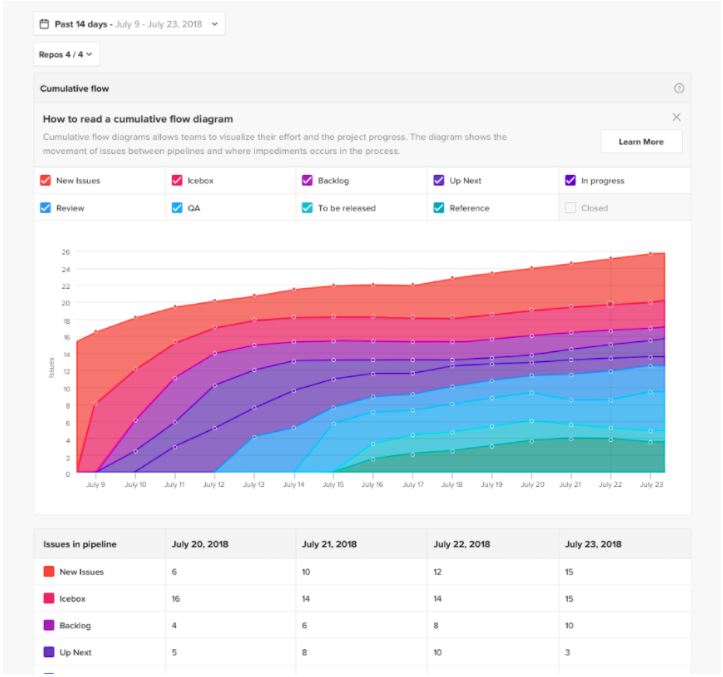
\includegraphics[width=1\textwidth]{cumulative_flow.PNG}
\caption{Gráfico Cumulative Flow}
\label{fig:cumulative}
\end{figure}

\section*{Control Charts Report}

Control Chart Report (CCR) proporciona el tiempo de ciclo y el tiempo de entrega,o el tiempo que tarda el equipo en resolver los problemas, ayudando a predecir la rapidez con la que se solucionán los problemas. Así como identificar cuellos de botella.

En la Figura \ref{fig:control} los puntos representan un problema cerrado. Un punto relleno representa un grupo de problemas cerrados. 

\begin{figure}[h!] 
\centering
    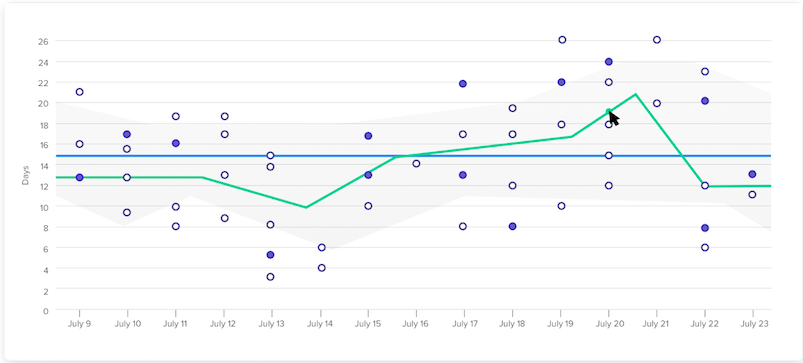
\includegraphics[width=1\textwidth]{control_chart.PNG}
\caption{Gráfico Control Chart}
\label{fig:control}
\end{figure}

El eje x marca la fecha en la que se completó el problema, y el eje y los días que tardó en completarse. La líea azul muestra el número medio de días que se tarda en cerrar una incidencia durante todo el período de tiempo seleccionado. La línea verde muestra un promedio móvil de la cantidad de días que lleva cerrar los problemas más recientes. 


\section*{Burndown Charts}

Los Burndown Charts son representaciones visuales simples del progreso actual del equipo en el sprint. Ofreciendo una visión inmediata del estado de su equipo.

\begin{itemize}
    \item El eje vertical muestra el esfuerzo total para completar el hito.
\end{itemize}

El eje horizontal muestra el tiempo en días.
Una lína ideal muestra como progresaría el proyecto a un ritmo constante (línea gris claro y discontinua).    
Una línea real que muestra los puntos restantes de hisotria a medida que el equipo avanza en el hito (línea morada y sólida).


\begin{figure}[h!] 
\centering
    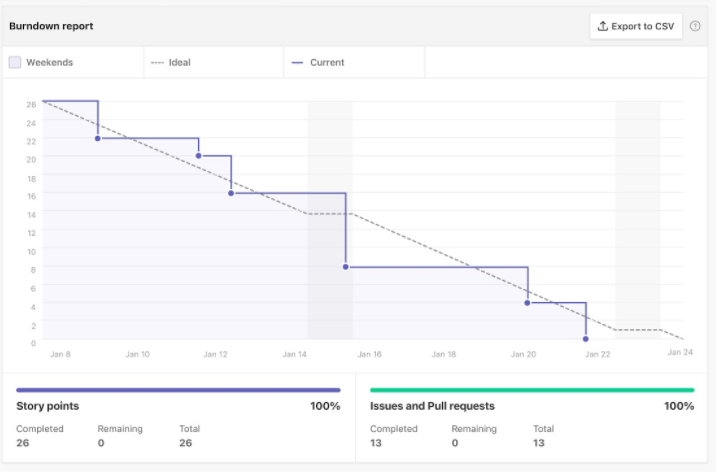
\includegraphics[width=1\textwidth]{burndown-chart.PNG}
\caption{Gráfico Burndown Chart}
\label{fig:control}
\end{figure}


\section*{Velocity Charts}

La velocidad del equipo es una "medida de la cantidad de trabajo que un equpo puede abordar durante un solo sprint y es la métrica clave en Scrup". Cuando finaliza un Sprint se sumará los puntos de todas las historias de usuario completadas y , con el tiempo, encontrará la cantidad promedio de punto por sprint (permite al equipo realizar estimacioens futuras para evitar problemas como no cumplir con la fecha límite).

\section*{Release Reports}

Los Release Reports son una forma de realizar un seguiemeinto de los proyectos a largo plazo, objetivos comerciales o compromisos externos, como el lanzamiento de una nueva función. Este informe proporciona una mejor perspectiva de las fechas de finalización previstaas y si está o no encaminado para finalizar el lanzamiento en la fecha de finalización deseada. 

Ofrecen mayor utilidad cuando se abarcan múltiples sprints, y trabajan múltiples equipos coordinados o se ven afectados por muchas partes móviles dentro de la organización.

\begin{figure}[h!] 
\centering
    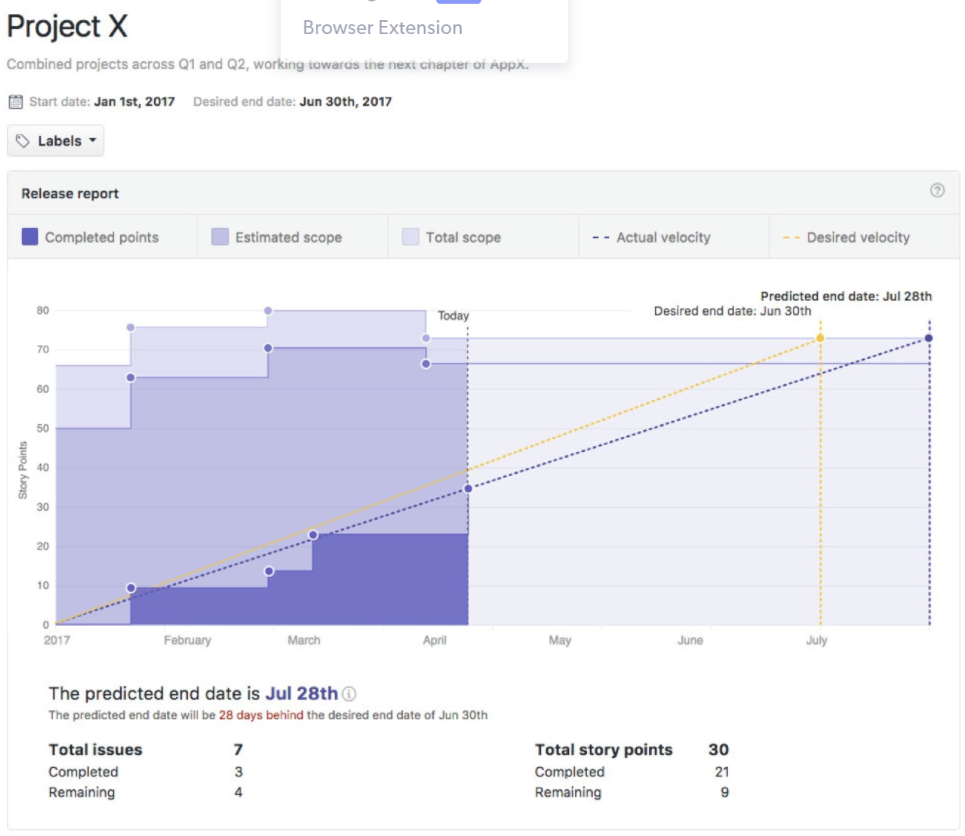
\includegraphics[width=1\textwidth]{release-report.PNG}
\caption{Gráfico Release Reports}
\label{fig:control}
\end{figure}


\bibliographystyle{plain}
\bibliography{library}


\end{document}